\documentclass[]{report}


\usepackage[a4paper, 
total={170mm,257mm},
left=20mm,
top=20mm,
]{geometry}

\usepackage[utf8]{inputenc}
\usepackage[portuges]{babel}
\usepackage{subcaption}
\usepackage{graphicx}
\usepackage{amsmath}
\usepackage{subfiles}
\usepackage{bm}

% Title Page
\title{Robô seguidor de linha}
\author{
	Daniel Barros\\
	\texttt{up201704271@fe.up.pt}
	\and
	Ricardo Falcão\\
	\texttt{up201704220@fe.up.pt}
}


\begin{document}
\maketitle

\section*{Introdução}
No âmbito da cadeira de SBMI, foi nos proposto o desenvolvimento de um robô seguidor de linha, utilizando para isso motores DC e sensores óticos. Neste relatório demonstraremos o nosso processo de desenvolvimento do projeto, assim como as conclusões que dele tiramos.

\section*{Arquitetura}
O robô projetado é dividido em 3 secções fundamentais: Recolha de informação, processamento dessa informação, e atuação por meio dos motores. Estas serão explicadas ao pormenor de seguida:

\subsection*{Recolha de informação}
Na recolha de informação foi utilizada um \textit{array} de 5 sensores IR, o CNY70. O esquema elétrico de cada sensor é o seguinte:

\begin{figure}[!htb]
	\centering
	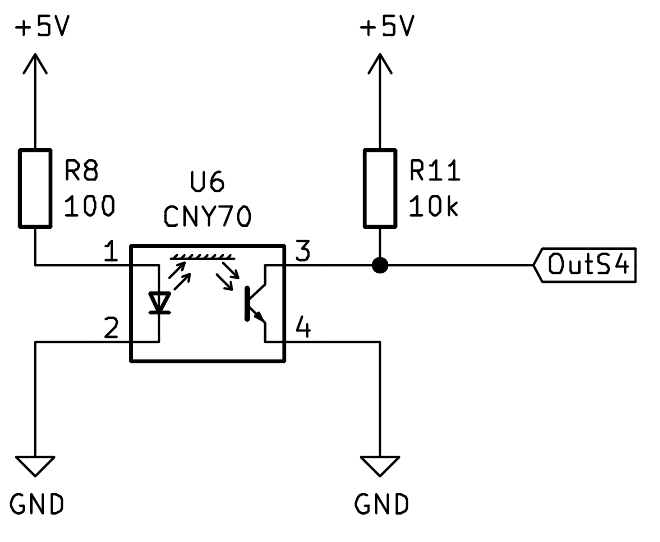
\includegraphics[width=5cm]{imagens/sensor}
	\caption{Sensores de linha (CNY70)}
\end{figure}

Perante esta configuração, era necessário uma corrente de 50 mA no LED emissor, e foi dimensionada então uma resistência limitadora de corrente de 100 $\Omega$; No coletor do foto-transístor estará uma tensão que varía com a intensidade de luz recebida. Quanto menor for a luz recebida, maior será a tensão $V_{out}$. \\
Será necessário, na pista, utilizar cores bastante diferentes no chão e na linha, para atingir a máxima resolução deste sensor. Nos nossos testes, foi utilizada uma pista de fundo branco com uma linha preta, mas o contrário era também admissível. \\
Devido ao elevado número de sinais analógicos a serem processados (que será abordado posteriormente), foi necessário utilizar um multiplexador analógico, nomeadamente o CD4051B. O seu esquema elétrico é o seguinte:

\begin{figure}[!htb]
	\centering
	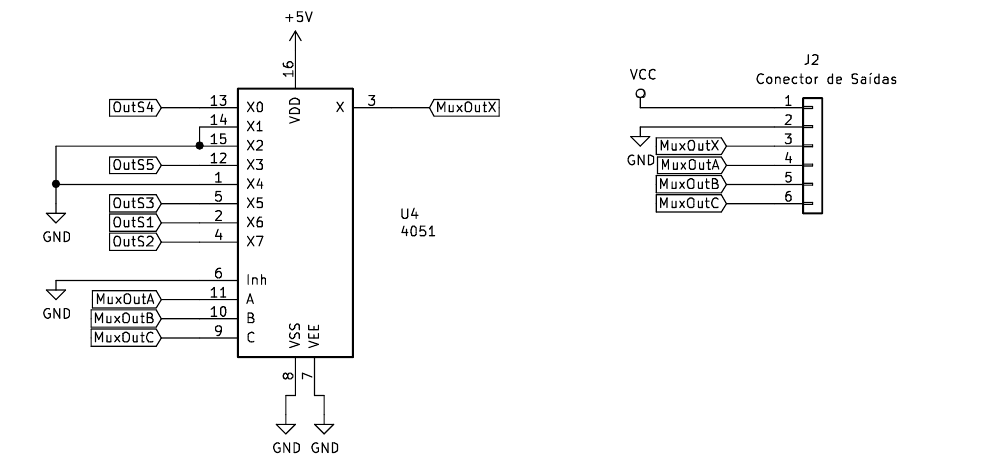
\includegraphics[width=14cm]{imagens/mux}
	\caption{Multiplexador analógico (CD4051B)}
\end{figure}

\pagebreak

\subsection*{Processamento de sinal}
Para o processamento de sinal foi utilizado o microcontrolador Atmega328p, numa placa Arduino Uno.
O processamento de sinal tem a seguinte sequência de passos:


\begin{figure}[!htb]
	\centering
	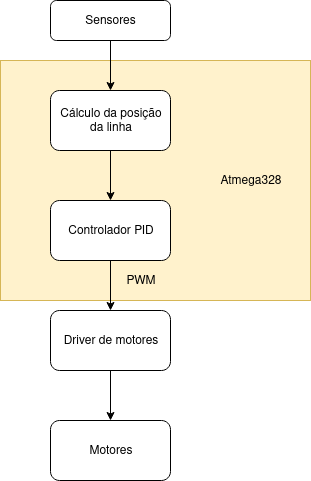
\includegraphics[width=5cm]{imagens/atmega_flow}
	\caption{Processamento de sinal (Atmega328)}
\end{figure}

Para o calculo da posição da linha é primeiro necessário recolher as tensões de saída dos sensores óticos. Estes devem ser calibrados no código para o valor digital mínimo que pode recolher assim como para o valor máximo. Cada leitura do sensor será transformada num número decimal, sendo 0 quando corresponde ao valor mínimo, e 1 no valor máximo. \\
Se para cada sensor atribuirmos o seguinte peso:

\end{document}          
